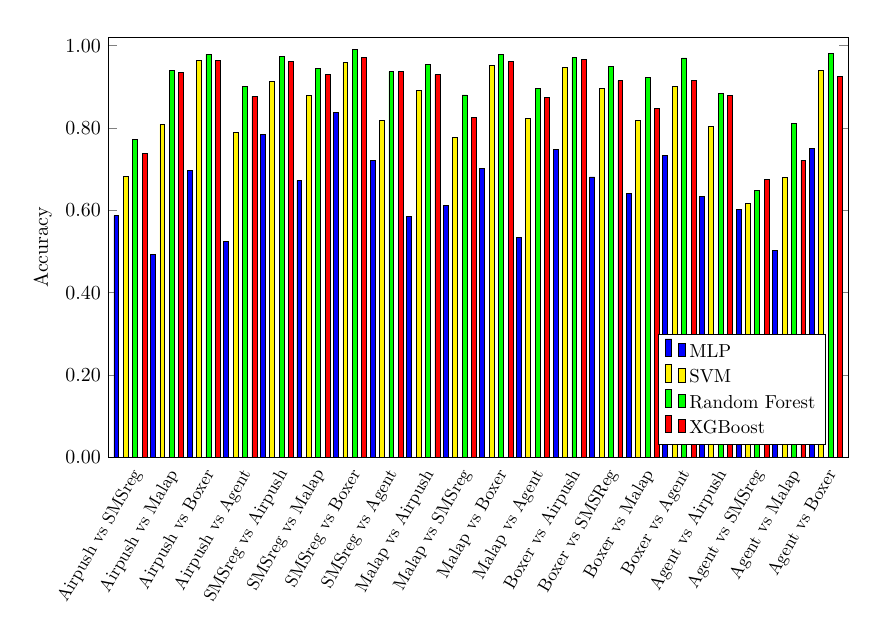
\begin{tikzpicture}[scale=0.8, every node/.style={scale=1.0}]
\pgfkeys{/pgf/number format/.cd,1000 sep={}}
\begin{axis}[%axis x line*=bottom,
	%bar shift=0pt,
        width  = 1.1*\textwidth,
        height = 8.25cm,
        ymin=0.0,ymax=1.02,
%        ytick={0.0, 0.1, 0.2, 0.3, 0.4, 0.5, 0.6, 0.7, 0.8, 0.9, 1.0},
        ytick={0.0, 0.2, 0.4, 0.6, 0.8, 1.0},
        major x tick style = transparent,
        ybar=5*\pgflinewidth,
%        bar width=15.0pt,
        bar width=2.25pt,
%        ymajorgrids = true,
%        xlabel = {Learning technique},
        ylabel = {Accuracy},
        ylabel style = {scale = 0.9},
%        symbolic x coords={MLR, SVC, MLP, CNN, RNN, LSTM, RF, XGBoost},
%        xticklabels={MLR, SVC, MLP, CNN, RNN, LSTM, RF, XGBoost},
        symbolic x coords={
        Airpush vs SMSreg, 
        Airpush vs Malap, 
        Airpush vs Boxer, 
        Airpush vs Agent, 
        SMSreg vs Airpush, 
        SMSreg vs Malap, 
        SMSreg vs Boxer, 
        SMSreg vs Agent, 
        Malap vs Airpush, 
        Malap vs SMSreg, 
        Malap vs Boxer, 
        Malap vs Agent, 
        Boxer vs Airpush, 
        Boxer vs SMSReg, 
        Boxer vs Malap, 
        Boxer vs Agent, 
        Agent vs Airpush, 
        Agent vs SMSreg, 
        Agent vs Malap, 
        Agent vs Boxer
        },
        xticklabels={
        Airpush vs SMSreg, 
        Airpush vs Malap, 
        Airpush vs Boxer, 
        Airpush vs Agent, 
        SMSreg vs Airpush, 
        SMSreg vs Malap, 
        SMSreg vs Boxer, 
        SMSreg vs Agent, 
        Malap vs Airpush, 
        Malap vs SMSreg, 
        Malap vs Boxer, 
        Malap vs Agent, 
        Boxer vs Airpush, 
        Boxer vs SMSReg, 
        Boxer vs Malap, 
        Boxer vs Agent, 
        Agent vs Airpush, 
        Agent vs SMSreg, 
        Agent vs Malap, 
        Agent vs Boxer
        },
	y tick label style={scale=0.9,
%		rotate=60,
    		/pgf/number format/.cd,
   		fixed,
   		fixed zerofill,
%		sep=,
    		precision=2},
%	yticklabel pos=right,
        xtick = data,
        x tick label style={scale=0.8,
        		rotate=60,
%		font=\small,
		anchor=north east,
		inner sep=0mm
		},
%		font=\small},
%        scaled y ticks = false,
	%%%%% numbers on bars and rotated
%        nodes near coords,
%        every node near coord/.append style={rotate=90, scale=0.75,
%        								   anchor=west, 
%								   %font=\footnotesize,
%								   /pgf/number format/.cd,
%								   fixed,
%								   fixed zerofill,
%%								   sep=,
%								   precision=4},
        %%%%%
%        enlarge x limits=0.03,
%        enlarge x limits=0.06,
        enlarge x limits=0.0325,
        legend cell align=left,
        legend pos=south east,
        legend style={nodes={scale=0.85},
%%                at={(1,1.05)},
%%                anchor=south east,
%%	        nodes={rotate=90},%%%%% rotate text in legend
%%                at={(0.125,0)},
%%                at={(0.125,0)},
%%                at={(0.8775,0)},
%                at={(0.82,0.56)},
%                anchor=south,
%                column sep=1ex
        },
]
\addplot [fill=blue,opacity=1.00]
coordinates {
(Airpush vs SMSreg, 0.5872)
(Airpush vs Malap,  0.4936)
(Airpush vs Boxer, 0.6956)
(Airpush vs Agent, 0.5240)
(SMSreg vs Airpush, 0.7833)
(SMSreg vs Malap, 0.6729)
(SMSreg vs Boxer, 0.8367)
(SMSreg vs Agent, 0.7217)
(Malap vs Airpush, 0.5854)
(Malap vs SMSreg, 0.6111)
(Malap vs Boxer, 0.7017)
(Malap vs Agent, 0.5346)
(Boxer vs Airpush, 0.7472)
(Boxer vs SMSReg, 0.6809)
(Boxer vs Malap, 0.6400)
(Boxer vs Agent, 0.7333)
(Agent vs Airpush, 0.6334)
(Agent vs SMSreg, 0.6022)
(Agent vs Malap, 0.5017)
(Agent vs Boxer, 0.7509)
};
\addlegendentry{MLP}
\addplot [fill=yellow,opacity=1.00]
coordinates {
(Airpush vs SMSreg, 0.6813)
(Airpush vs Malap, 0.8086)
(Airpush vs Boxer, 0.9644)
(Airpush vs Agent, 0.7883)
(SMSreg vs Airpush, 0.9121)
(SMSreg vs Malap, 0.8781)
(SMSreg vs Boxer, 0.9588)
(SMSreg vs Agent, 0.8186)
(Malap vs Airpush, 0.8906)
(Malap vs SMSreg, 0.7774)
(Malap vs Boxer, 0.9511)
(Malap vs Agent, 0.8220)
(Boxer vs Airpush, 0.9464)
(Boxer vs SMSReg, 0.8954)
(Boxer vs Malap, 0.8174)
(Boxer vs Agent, 0.9017)
(Agent vs Airpush, 0.8039)
(Agent vs SMSreg, 0.6165)
(Agent vs Malap, 0.6800)
(Agent vs Boxer, 0.9400)
};
\addlegendentry{SVM}
\addplot [fill=green,opacity=1.00]
coordinates {
(Airpush vs SMSreg, 0.7726)
(Airpush vs Malap, 0.9391)
(Airpush vs Boxer, 0.9788)
(Airpush vs Agent, 0.9009)
(SMSreg vs Airpush, 0.9743)
(SMSreg vs Malap, 0.9436)
(SMSreg vs Boxer, 0.9898)
(SMSreg vs Agent, 0.9367)
(Malap vs Airpush, 0.9549)
(Malap vs SMSreg, 0.8800)
(Malap vs Boxer, 0.9777)
(Malap vs Agent, 0.8951)
(Boxer vs Airpush, 0.9701)
(Boxer vs SMSReg, 0.9499)
(Boxer vs Malap, 0.9220)
(Boxer vs Agent,  0.9699)
(Agent vs Airpush, 0.8843)
(Agent vs SMSreg, 0.6487)
(Agent vs Malap, 0.8109)
(Agent vs Boxer, 0.9817)
};
\addlegendentry{Random Forest}
\addplot [fill=red,opacity=1.00]
coordinates {
(Airpush vs SMSreg, 0.7378)
(Airpush vs Malap, 0.9348)
(Airpush vs Boxer, 0.9632)
(Airpush vs Agent, 0.8764)
(SMSreg vs Airpush, 0.9612)
(SMSreg vs Malap, 0.9307)
(SMSreg vs Boxer, 0.9717)
(SMSreg vs Agent, 0.9364)
(Malap vs Airpush, 0.9297)
(Malap vs SMSreg, 0.8251)
(Malap vs Boxer, 0.9614)
(Malap vs Agent, 0.8740)
(Boxer vs Airpush, 0.9655)
(Boxer vs SMSReg, 0.9145)
(Boxer vs Malap, 0.8464)
(Boxer vs Agent, 0.9151)
(Agent vs Airpush, 0.8783)
(Agent vs SMSreg, 0.6748)
(Agent vs Malap, 0.7217)
(Agent vs Boxer, 0.9252)
};
\addlegendentry{XGBoost}
\end{axis}
\end{tikzpicture}
